\chapter{Requirement analysis and Software design}

\label{ch:Requirement analysis and Software design}

\setlength{\parindent}{4em} \setlength{\parskip}{1em} \global\long\def\baselinestretch{1.5}



\section{Requirement for application}


\subsection{Functional requirement}
\begin{itemize}
\item The system allows user to control machine using brainwave. 
\item The system allows user to check the EEG headset status. 
\item The system allows administrator to see the authentication result. 
\item The system allows administrator to see real-time graph of each band. 
\item The system allows administrator to check the EEG headset status. 
\item The system allows user to save information into the system. 
\item The system shows the analysis result. 
\end{itemize}
\newpage{}


\subsection{Non-Functional requirement}
\begin{itemize}
\item The system uses C\# language to develop software. 
\item The system uses Windows Presentation form and Visual studio to create
user interface. 
\item User friendly: The UI is look clear, simple, easy to use and understand. 
\item Performance: The system shows and records the EEG brainwave in real-time. 
\end{itemize}

\section{Use case Diagram}

\begin{figure}[ht]
\centering 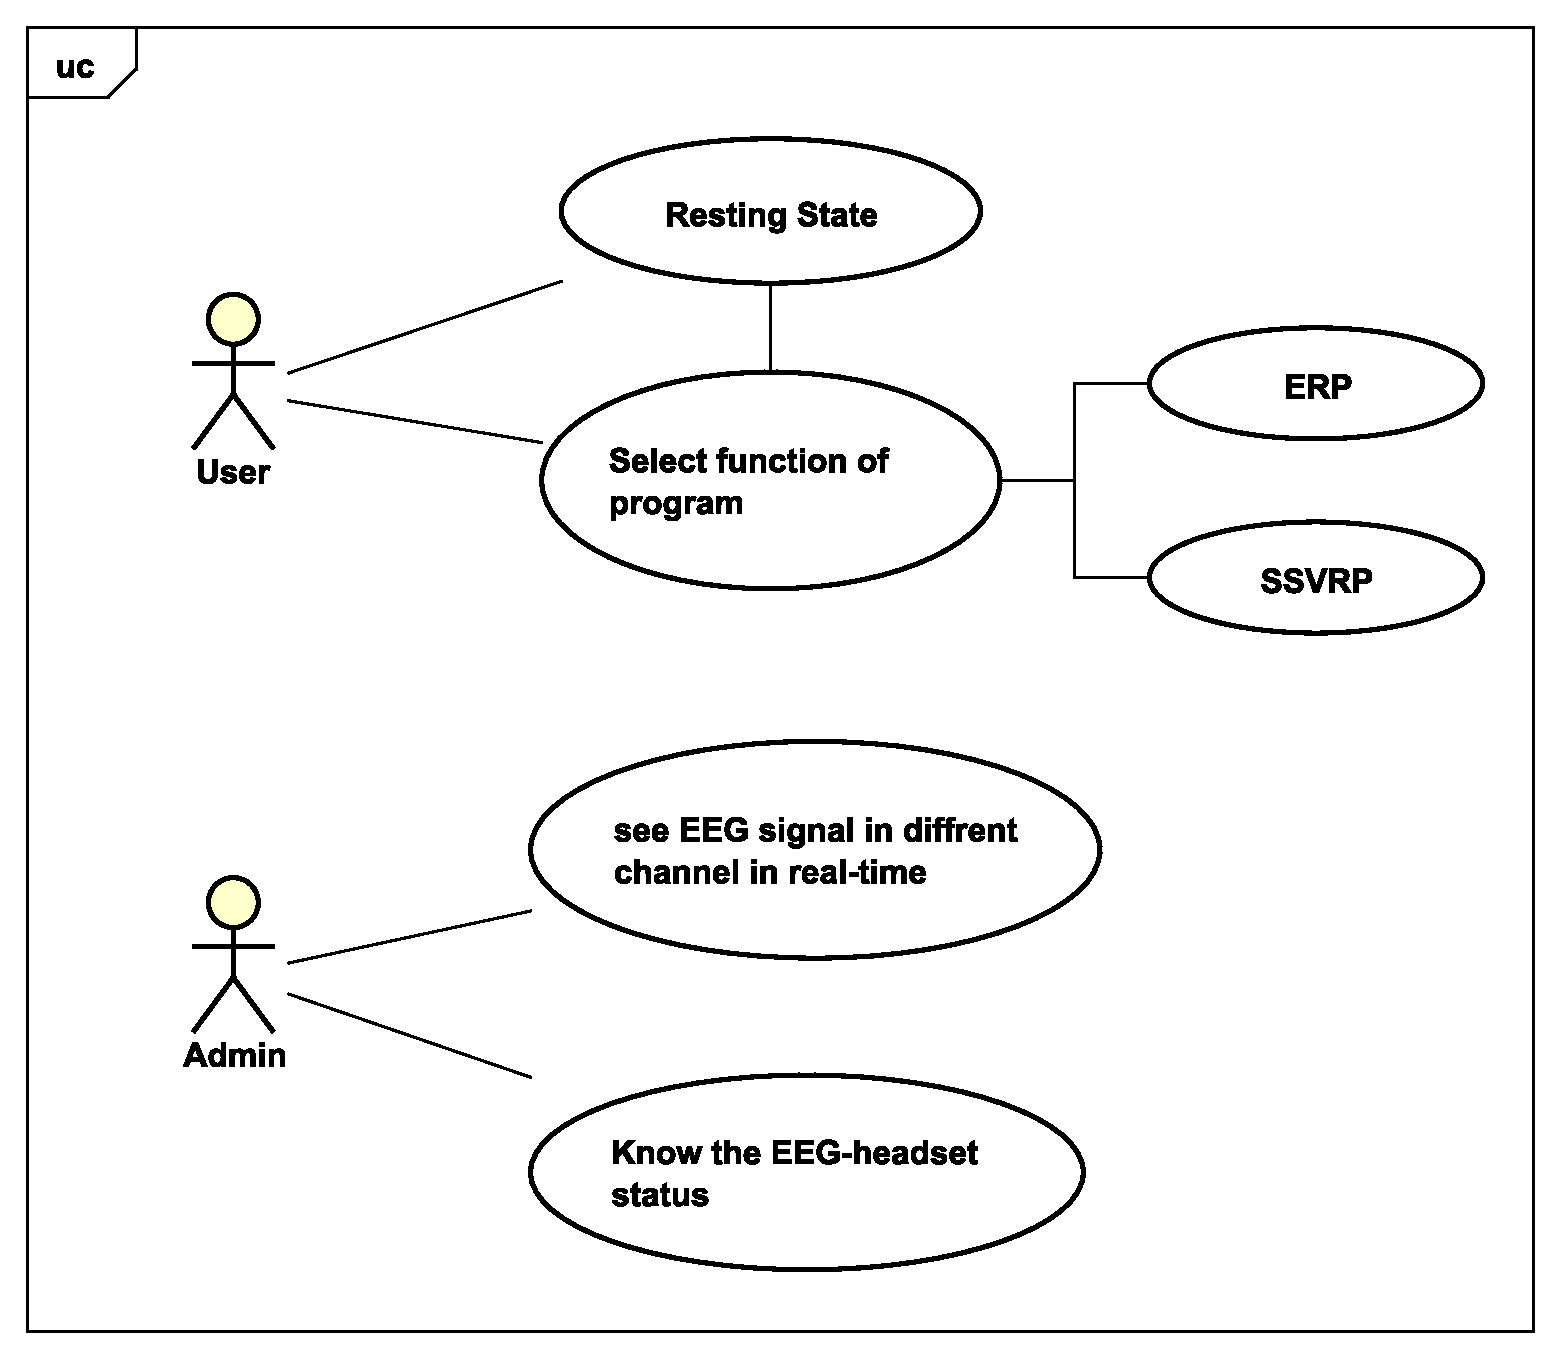
\includegraphics[scale=0.5]{chapter4/uc.pdf}
\caption{Use case diagram}
\end{figure}


\newpage{}


\subsection{Use case description for user and admin}
\begin{itemize}
\item \textbf{Expanded description of "Know the EEG-headset status
use case" }

\begin{description}
\item [{Use case:}] Know the EEG-headset status 
\item [{Actor:}] Admin 
\item [{Goal:}] To make sure that the Emotiv headset will record EEG with
the proper signal. 
\item [{Overview:}] The admin will equip the Emotiv headset on the subject(user)
head then observes the EEG-headset status to make sure that Emotiv
headset will record SSVEP with the proper signal for the starting
program for subject. 
\item [{Typical course of events:}]~

{
	\centering

\begin{tabular*}[\textwidth]{ | C | C | }
	
\hline 
\textbf{User} & \textbf{System}  \tabularnewline
\hline 
1. Subject asks admin to access the system & cell5  \tabularnewline
\hline 
2. Subject is equipped the Emotiv headset by admin  & cell8  \tabularnewline
\hline 
\end{tabular}
}

\end{description}
\item Another entry in the list 
\end{itemize}

\section{Activity Diagram}


\subsection{Activity diagram of resting state}

\begin{figure}[ht]
\centering 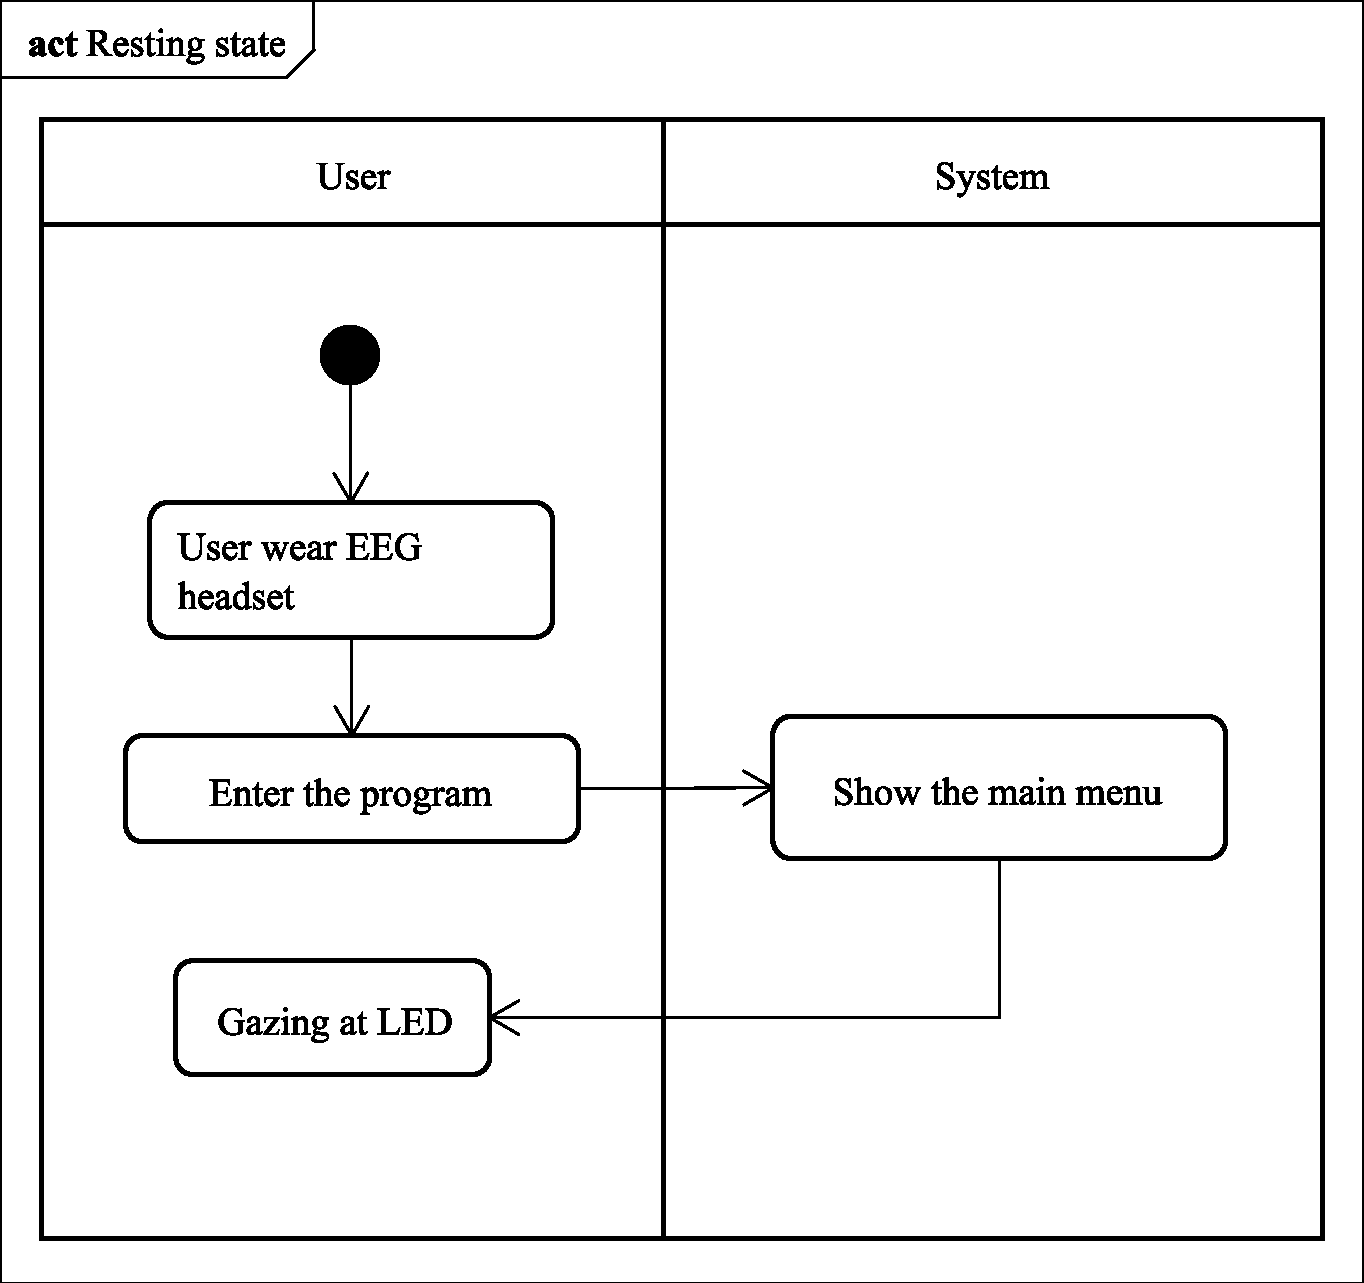
\includegraphics[scale=0.295]{chapter4/Rest.pdf}
\caption{Activity diagram of resting state}
\end{figure}



\subsection{Activity diagram of ERP}

\begin{figure}[ht]
\centering 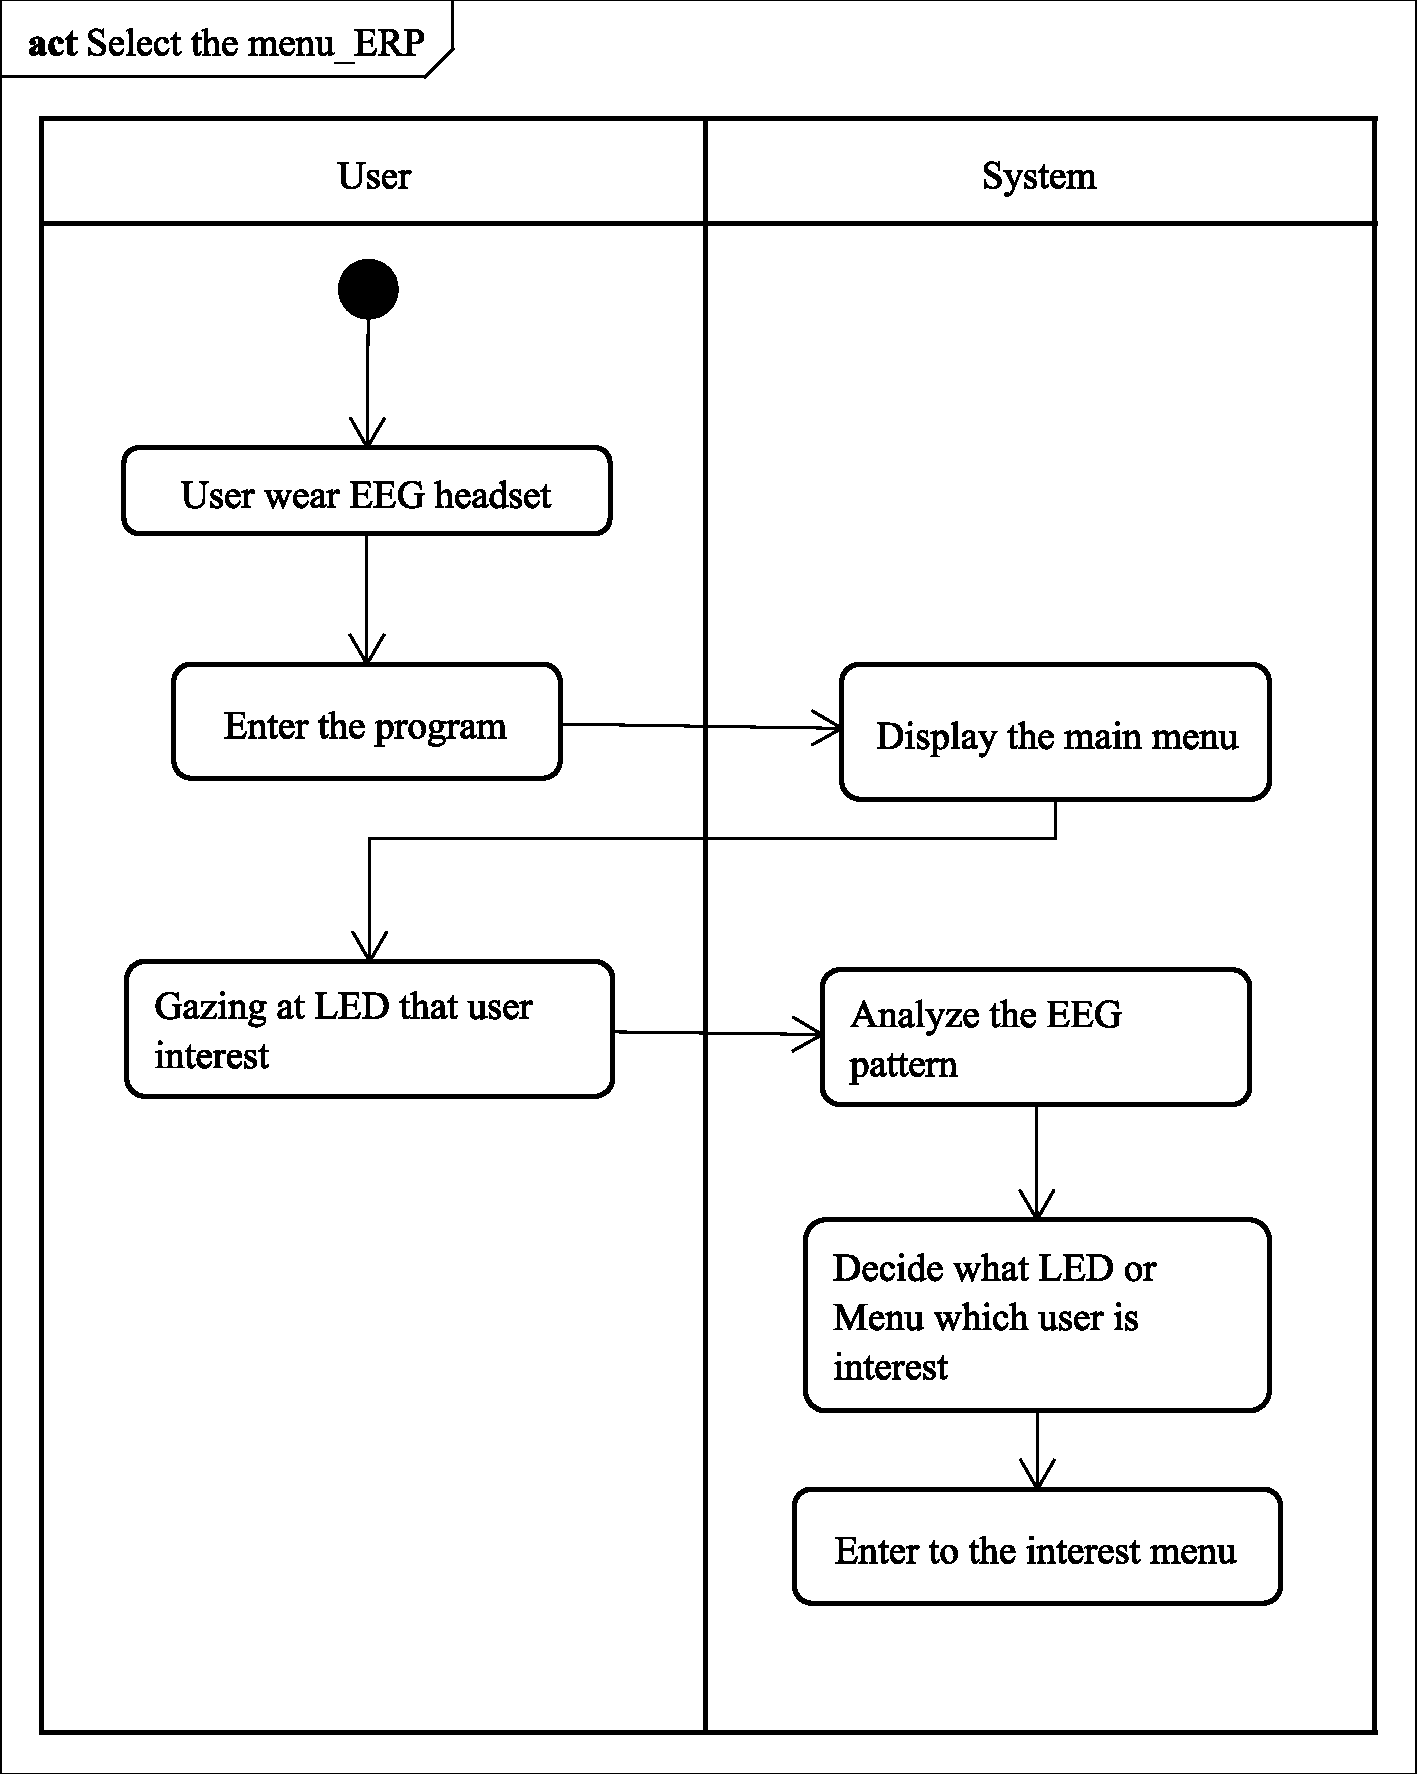
\includegraphics[scale=0.295]{chapter4/av_ERP.pdf}
\caption{Activity diagram of ERP}
\end{figure}


\newpage{}


\subsection{Activity diagram of SSVEP}

\begin{figure}[ht]
\centering 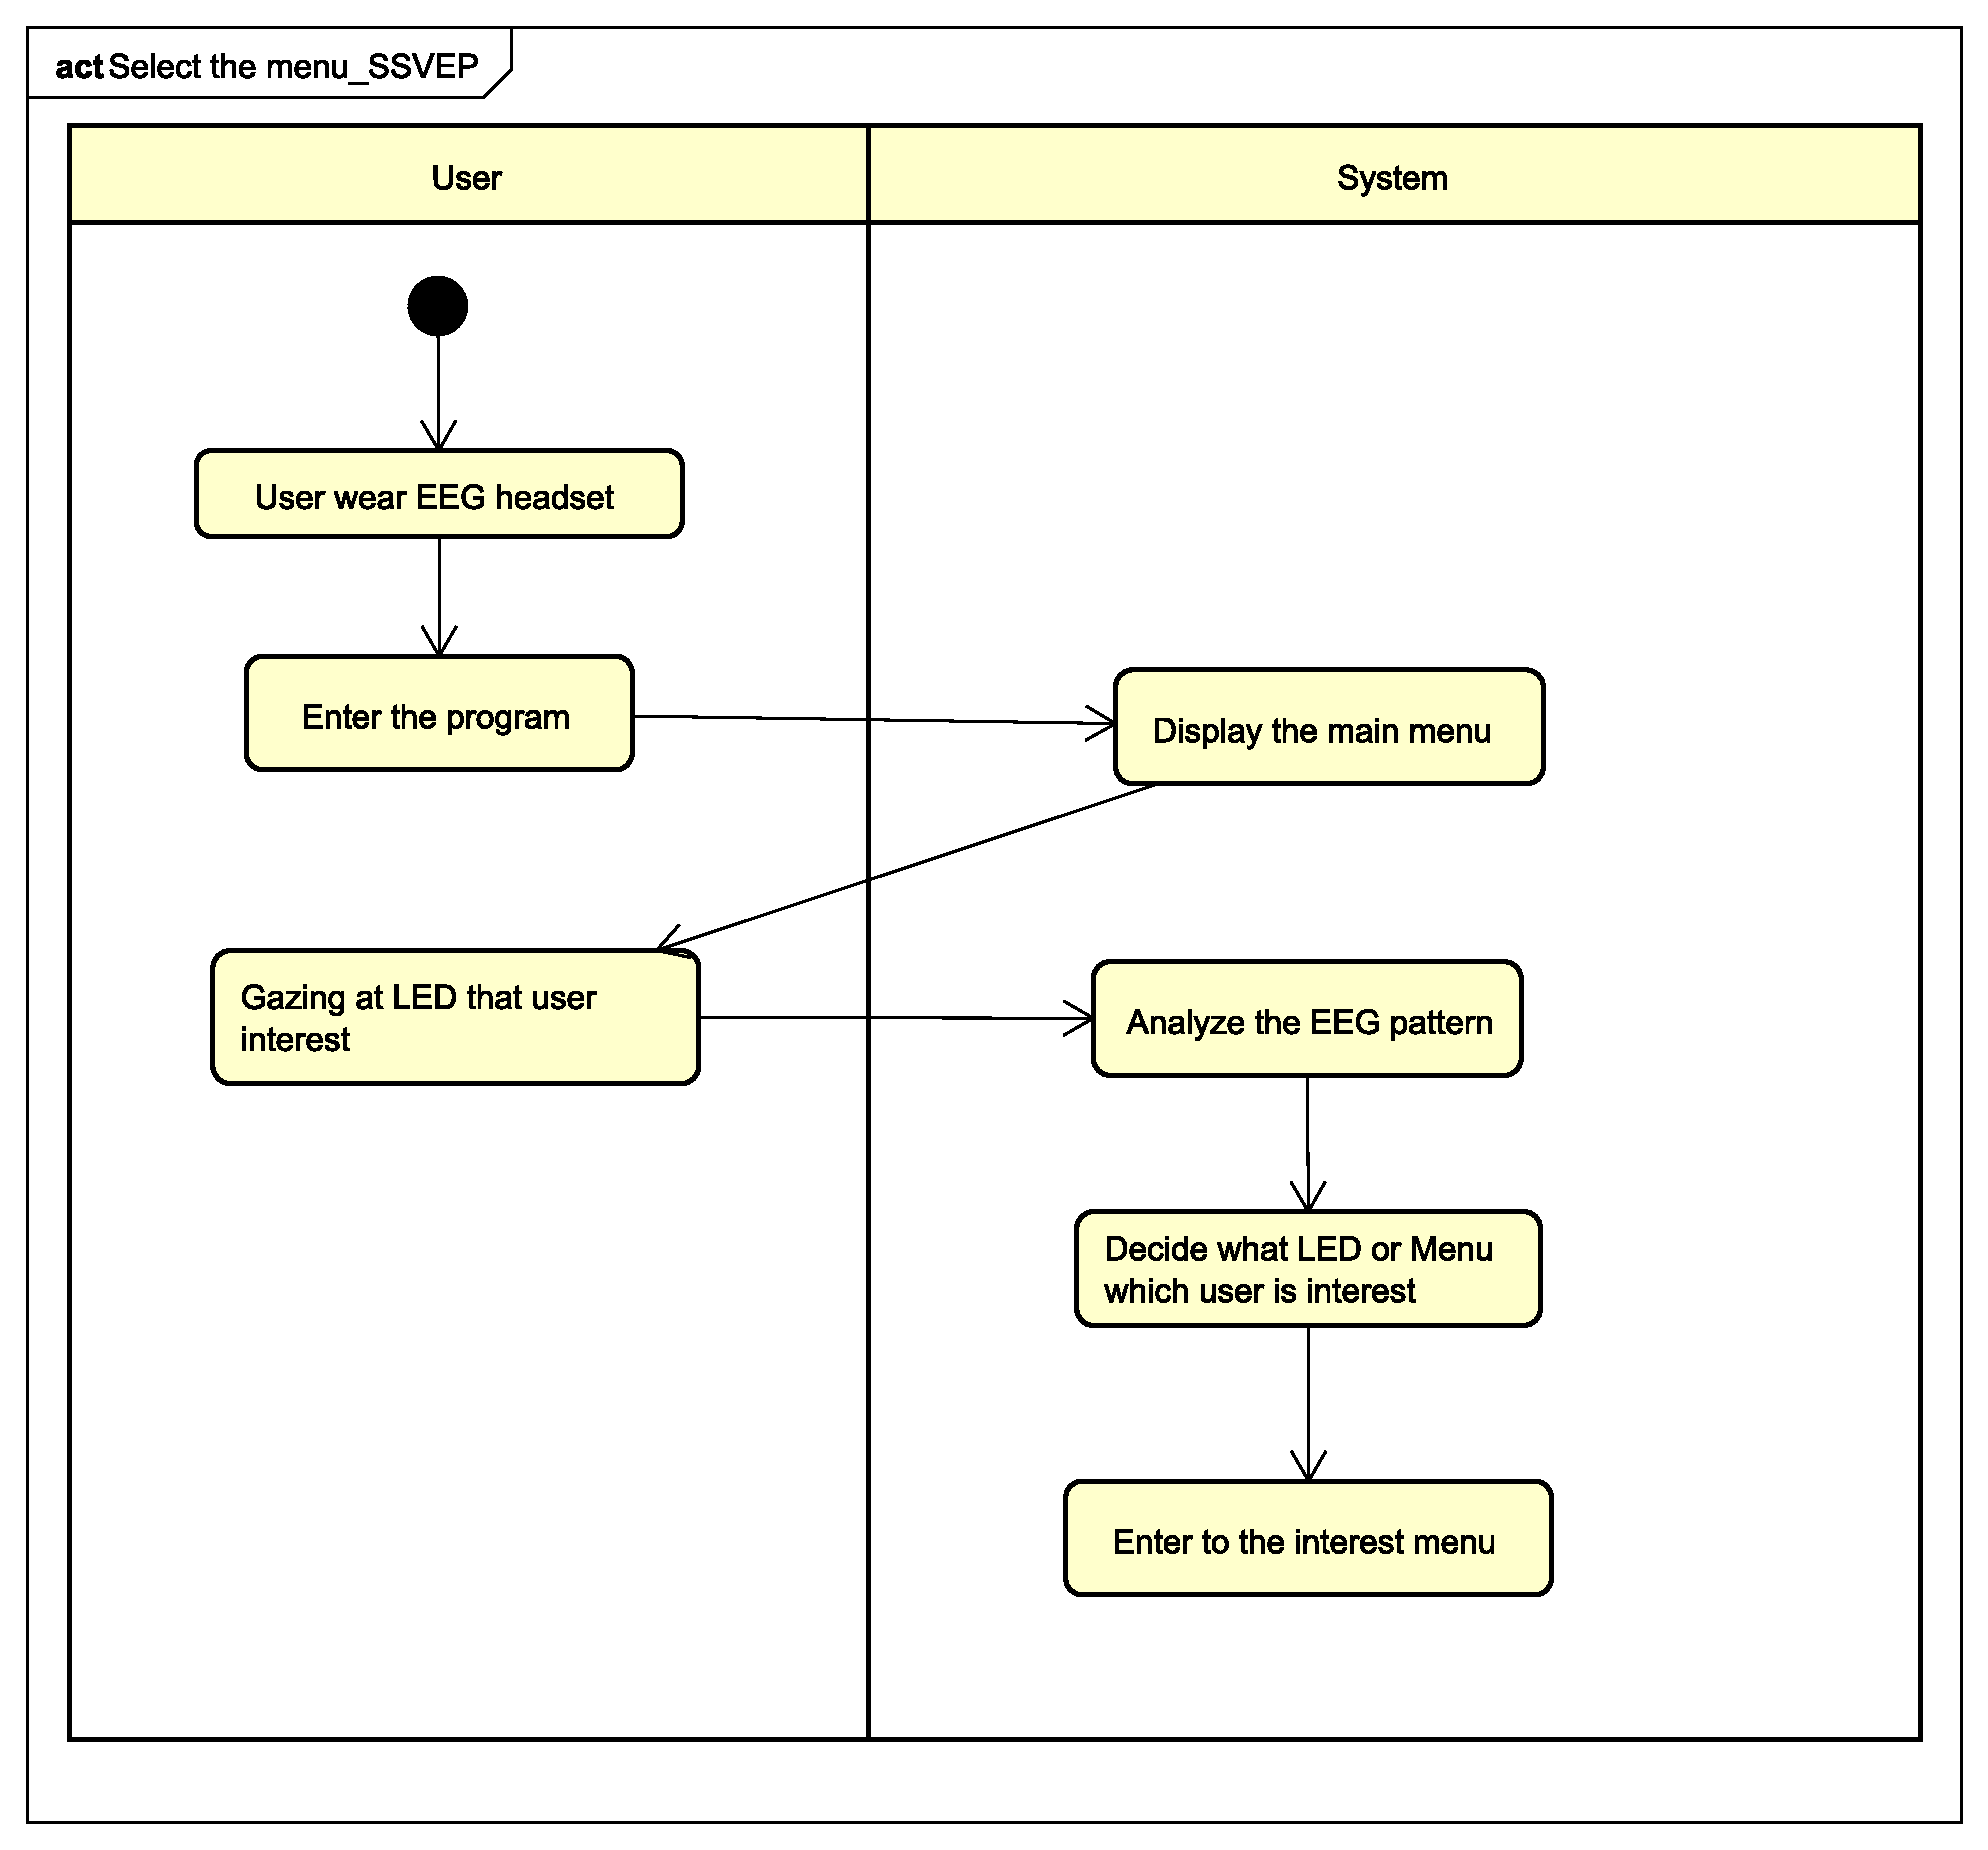
\includegraphics[scale=0.295]{chapter4/av_SSVEP.pdf}
\caption{Activity diagram of SSVEP}
\end{figure}

